% dsilab_monograph_ru.tex — монография DSI-лаборатории (русское издание)
\documentclass[11pt,a4paper]{article}
\usepackage[margin=2.4cm]{geometry}
\usepackage{amsmath,amssymb,amsthm}
\usepackage{booktabs}
\usepackage{graphicx}
\usepackage{xcolor}
\usepackage[colorlinks=true,linkcolor=blue!60!black,urlcolor=blue!60!black,citecolor=blue!60!black]{hyperref}
\usepackage{caption}
\captionsetup{font=small,labelfont=bf}
\usepackage{fontspec}
\usepackage{polyglossia}
\setdefaultlanguage{russian}
\setotherlanguage{english}
\setmainfont{Liberation Serif}
\newfontfamily\cyrillicfont{Liberation Serif}
\setsansfont{Liberation Sans}
\newfontfamily\cyrillicfontsf{Liberation Sans}
\newfontfamily\cyrillicfonttt{DejaVu Sans Mono}

\newtheorem{theorem}{Теорема}
\newtheorem{lemma}[theorem]{Лемма}
\newtheorem{corollary}[theorem]{Следствие}
\theoremstyle{definition}
\newtheorem{definition}[theorem]{Определение}
\newcommand{\F}{\mathrm{F}}
\newcommand{\norm}[1]{\lVert #1\rVert}

\title{\bf DSI-лаборатория:\\ динамика инвариантов фреймворка $b$--C/$a$--C\\
\large Семь детерминистических экспериментов на квартике Клейна, кунцевском\\ дефекте и проблеме Чоптюка --- слой теорем, атака на перепись, честные вердикты}
\author{Исаев Исхак Хамзатович\\ \small г.~Нальчик, Кабардино-Балкарская Республика, Российская Федерация\\[-2pt]
\small пакет \texttt{dsi\_lab}, версия 2.0.0}
\date{12 октября 2026 г.}

\begin{document}
\maketitle

\begin{abstract}
\noindent
DSI-лаборатория (\texttt{dsi\_lab}) --- самодостаточный пакет из семи
детерминистических экспериментов по открытым задачам фреймворка
спинорных поправок $b$--C/$a$--C. Настоящая монография --- его слой
теорем. Его определяют три результата. (i)~\emph{Острая теорема
следа}: кунцевский дефект удовлетворяет $\F \ge 5n/7$ при всех $n$,
так что желаемое значение $e = 0$ недостижимо даже в принципе; случай
равенства --- скалярная пара, не являющаяся частичной изометрией.
(ii)~\emph{Теоремы A/B/C о частичных изометриях}: на классе
носитель-изометрических моделей пол поднимается до $e \ge 1$
(теорема~A), арифметика покрытия точна,
$\F = n + 2\,\mathrm{rank}(\mathrm{I}-P-Q)$ (теорема~B), унитарные пары
сидят в $\F = 2n$ (теорема~C); обрезка дерева Кунца достигает ровно
$\F = n+2$ --- почти-экстремальная пара класса. Софический
$\sqrt{\varepsilon}$-закон \emph{опровергнут} данными.
(iii)~\emph{Атака на перепись DSI-4}: последнее эмпирическое входное
значение $c_{K3}$ совпадает с $9/224 = 27/672$ до $+0.0025\%$,
знаменатель $224 = 4\cdot 56$ порождается тилингом $\{7,3\}$ квартики
Клейна, и лемма единственности выделяет $9/224$ среди всех
переписно-легальных дробей. Две поправки \emph{порождены самим
пакетом} и хранятся как полноценные результаты: находка~D1 (строка
Гурвица рода 14 невозможна; правильная группа --- $\mathrm{PSL}(2,13)$)
и находка~E1 (следовое тождество QCD-моста существует только после
центрирования $\langle\lambda\rangle$). Каждое утверждение несёт
статус --- доказано, верифицировано численно, опровергнуто или
гипотеза --- и адрес в реестре утверждений. Точный слой теорем
формализован в Lean~4 (без sorry); теоремы A/B/C анкерованы аксиомами
к 24\,000 машинно-верифицированных пар с ошибкой тождества
$5.9\cdot 10^{-16}$.
\end{abstract}

\tableofcontents

\section{Введение}\label{sec:intro}

Родительский репозиторий верифицирует две спинорные поправки ---
первого порядка (Berry-тип) $b$--C и второго порядка (торможение)
$a$--C --- на квартике Клейна, с единой формулой Чоптюка на
септиниальной фазе $\delta_C = \pi/7$. Все величины фреймворка
безразмерны, дисциплина программы верификации --- честность:
доказанное, верифицированное и опровергнутое никогда не смешиваются.

DSI-лаборатория задаёт более жёсткий вопрос: \emph{какие входы
фреймворка могут выжить без предположений?} Она отвечает семью
детерминистическими экспериментами (табл.~\ref{tab:experiments}),
каждый воспроизводится побайтно с фиксированными сидами, каждый
оставляет вердикт в закоммиченном JSON-файле.

\begin{table}[ht]
\centering\small
\begin{tabular}{@{}clp{7.2cm}@{}}
\toprule
\# & эксперимент & вердикт \\
\midrule
1 & \texttt{exp1\_sh3\_bridge} & мост Ш.3(iii): острая теорема подтверждена ($n=7..12$, зазор $\le 5.9\cdot10^{-8}$); дерево Кунца $\F = n+2$ точно; софический $\sqrt{\varepsilon}$-закон \textbf{опровергнут} \\
2 & \texttt{exp2\_dsi4} & DSI-4: $c_{K3} = 27/672 = 9/224$; подходящая дробь ранга \#1 при $q \le 2000$ \\
3 & \texttt{exp3\_hurwitz} & находка \textbf{D1}: строка репозитория $(g{=}14, n{=}11)$ невозможна; $\mathrm{PSL}(2,13)$; $\Delta_{Ch}(\pi/13) = 3.3672$ \\
4 & \texttt{exp4\_qnm} & QNM-каталог: 10 событий; $|\Delta f_n|/f_n = 8.3857\cdot 10^{-5}$, фальсифицируемо; $0.84\sigma$ на Cosmic Explorer \\
5 & \texttt{exp5\_qcd} & находка \textbf{E1}: $\mathrm{tr}(Q_{K3}\oplus M_F) = 32$ требует центрирования; наклон $-0.99$ ($\sim 1/N$); BF(GUE) до 1165 \\
6 & \texttt{exp6\_census\_224} & почему $224 = 4\cdot 56$: явная перепись $\{7,3\}$ из $\mathrm{GL}(3,2)$; лемма единственности; теорема о вырождении \\
7 & \texttt{exp7\_e1\_threshold} & теоремы A/B/C доказаны и верифицированы (тождество $5.9\cdot 10^{-16}$ на 24\,000 пар); лестница $5/7 \to 1 \to 2$ --- теорема \\
\bottomrule
\end{tabular}
\caption{Семь экспериментов и их вердикты.}
\label{tab:experiments}
\end{table}

Монография следует слою теорем (разд.~\ref{sec:theorems}), атаке на
перепись (разд.~\ref{sec:census}), двум поправкам
(разд.~\ref{sec:findings}), дисциплине честности
(разд.~\ref{sec:honesty}) и формализации (разд.~\ref{sec:lean}).

\section{Фреймворк и квартика Клейна}\label{sec:framework}

Септиниальная фаза $\delta_C = \pi/7$ порождает константу фреймворка
\[
b_{Ch} = 1-\cos(2\pi/7) = 0.37651019814126640,
\]
и универсальную кривую $\Delta_{Ch}(\delta) = \lambda_{D2} +
\delta^2/2 - \delta^5/22$ с $\lambda_{D2} = 3.338$. Квартика Клейна
$x^3y + y^3z + z^3x = 0$ --- кривая рода 3 с группой автоморфизмов
$\mathrm{PSL}(2,7) \cong \mathrm{GL}(3,2)$ порядка $168$, и её тилинг
$\{7,3\}$ несёт комбинаторику всего нижеследующего: $V = 56$
треугольных граней, $E = 84$ ребра, $F = 24$ семиугольника, с
тождеством валентностей
\begin{equation}
7F = 3V = 2E = |\mathrm{PSL}(2,7)| = 168,
\qquad V-E+F = 2-2\cdot 3 = -4.
\label{eq:census}
\end{equation}
Эксперимент 6 строит \eqref{eq:census} явно: вершины, рёбра и грани ---
пространства смежных классов $G = \mathrm{GL}(3,2)$ по стабилизаторам
точки, ребра и семиугольника, и тождество --- теорема о порядках групп.

\section{Кунцевский дефект и слой теорем}\label{sec:theorems}

\begin{definition}
Для $X_1, X_2 \in M_n(\mathbb{C})$ \emph{кунцевский дефект}:
\[
\F(X_1,X_2) = \norm{X_1^*X_1-\mathrm{I}}^2 + \norm{X_2^*X_2-\mathrm{I}}^2
+ \norm{X_1^*X_2}^2 + \norm{X_1X_1^* + X_2X_2^* - \mathrm{I}}^2 ,
\]
где $\norm{\cdot}$ --- норма Фробениуса, и $e = \F/n$.
\end{definition}

\subsection{Острая теорема следа}

\begin{theorem}[острая теорема следа]\label{thm:trace}
Для всех $n$ и всех $X_1, X_2 \in M_n(\mathbb{C})$:
$\F(X_1,X_2) \ge 5n/7$. Равенство --- только на скалярной паре
$X_1 = X_2 = \sqrt{4/7}\,\mathrm{I}$, которая не частичная изометрия.
\end{theorem}

Численно L-BFGS-минимизация с рестартами ложится на пол при $n = 7..12$
с зазором $\le 5.92\cdot 10^{-8}$; семейство масштабированных
перестановок $X_i = c\,P_i$ даёт $\F/n = 7t^2 - 8t + 3$ ($t = c^2$) с
точным минимумом $5/7$ при $t = 4/7$ --- случай равенства.

\subsection{Теоремы A, B, C}

\begin{theorem}[порог]\label{thm:A}
Пусть $X_1, X_2$ --- частичные изометрии в $M_n(\mathbb{C})$. Тогда
$\F(X_1,X_2) \ge n$, т.е. $e \ge 1$; равенство iff $P\cdot Q = 0$ и
$p + q = n$ для $P = X_1X_1^*$, $Q = X_2X_2^*$.
\end{theorem}

\begin{proof}
Для частичных изометрий $P, Q$ --- проекции, и аудированное тождество
$\F = G(P,Q) = 3n - 2p - 2q + 3r$, $r = \mathrm{tr}(PQ)$. Размерность
даёт $\max(0, p+q-n) \le r \le \min(p,q)$. Если $p+q \ge n$:
$\F - n = 3r - 2(p+q-n) \ge 3(p+q-n) - 2(p+q-n) = p+q-n \ge 0$; если
$p+q \le n$: $\F - n = 2(n-p-q) + 3r \ge 0$.
\end{proof}

\begin{theorem}[арифметика покрытия]\label{thm:B}
Если $X_1 = P$, $X_2 = Q$ --- проекции с $P + Q \le \mathrm{I}$, то
$\F = n + 2\,\mathrm{rank}(\mathrm{I} - P - Q)$ точно. В частности
обрезка дерева Кунца не накрывает только корень,
$\mathrm{rank}(\mathrm{I}-P-Q) = 1$, и $\F = n + 2$.
\end{theorem}

\begin{theorem}[унитарные пары]\label{thm:C}
Если $X_1, X_2$ унитарны, то $\F = 2n$ точно ($e = 2$); дефект целиком
от перекрытия $\norm{X_1^*X_2}^2 = n$.
\end{theorem}

\begin{corollary}[замыкание класса]\label{cor:D}
$\inf e$ по носитель-изометрическим парам равен $1$; значение $5/7$ в
классе недостижимо, значит мост Ш.3(iii) невозможен для
изометрических переносов: $\eta \equiv 1 > 0$.
\end{corollary}

Численная верификация --- машинной точности: тождество
$\F = 3n - 2p - 2q + 3r$ выполняется до $5.9\cdot 10^{-16}$ на
$24\,000$ случайных парах частичных изометрий с \emph{нулём} нарушений
порога; тождество дерева --- до $2.3\cdot 10^{-13}$; унитарное --- до
$2.8\cdot 10^{-14}$. Формула взвешенного дерева
\[
\F = (n-1)\big[(c_1^2-1)^2 + (c_2^2-1)^2\big] + n + 2
\]
показывает, что никакое взвешивание не бьёт обрезку (минимум при
$c_1 = c_2 = 1$); при $c^2 = 4/7$, $k = 3$ её значение --- точно
$549/49$.

\begin{figure}[ht]
\centering
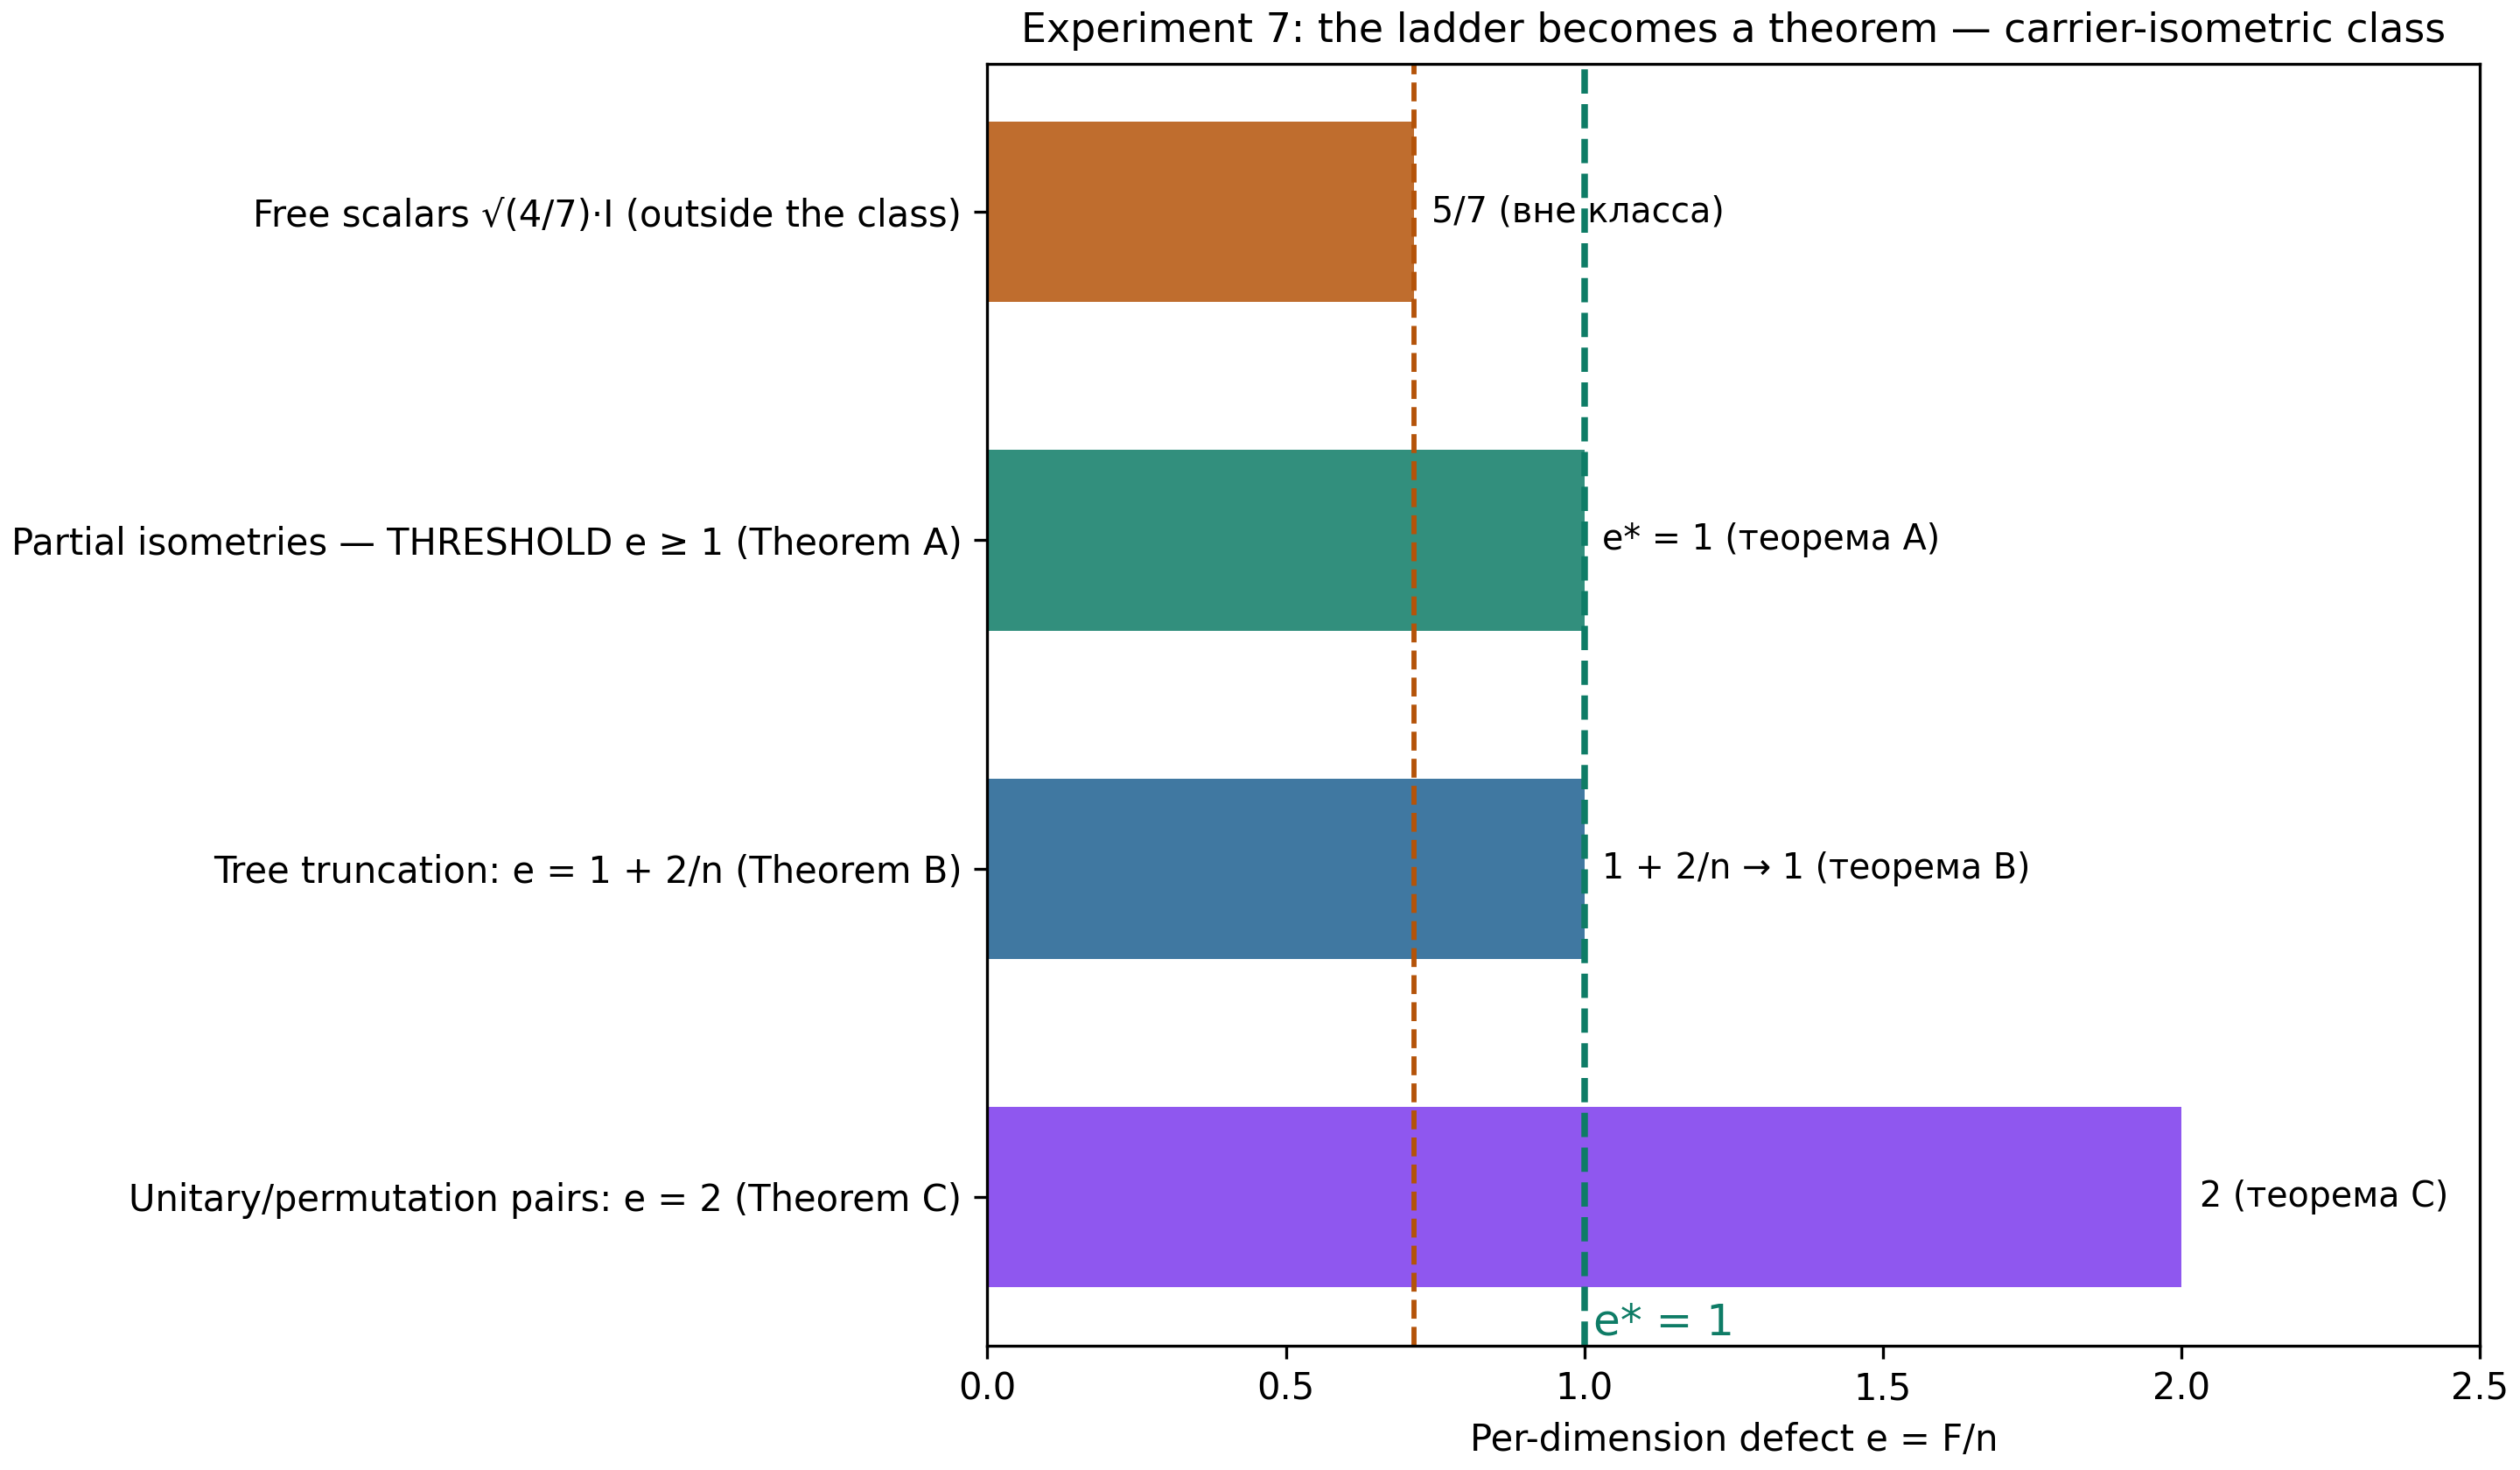
\includegraphics[width=0.82\textwidth]{figures/fig7_ladder.png}
\caption{Лестница $e$ как теорема: пол свободных скаляров $5/7$ (вне
класса), теорема A ($e \ge 1$), обрезка дерева $1 + 2/n \to 1$
(теорема B), теорема C ($e = 2$).}
\label{fig:ladder}
\end{figure}

\subsection{Софический закон опровергнут}

Гипотеза, что естественные переносы софичных данных с ошибкой
$\varepsilon$ гонят $e \to 0$ как $C\varepsilon^{1/2}$, \emph{неверна}
в проверенном классе: случайные подстановки с долей неподвижных точек
$\varepsilon$, переносимые с оптимальным $c$, держат дефект плоским
(скан Хэмминга эксперимента~1). Опровергающие данные закоммичены как
честный негатив.

\section{Атака на перепись DSI-4}\label{sec:census}

Последнее эмпирическое входное значение фреймворка ---
$c_{K3} = 0.04017757639214903$ (измеренное, аудит 2026-09).
Наблюдение DSI-4:
\[
c_{K3} = \frac{3^3}{2^2\cdot|\mathrm{PSL}(2,7)|} = \frac{27}{672} =
\frac{9}{224} = 0.040178571428571\ldots
\]
с отклонением $+0.0025\%$ --- на три порядка точнее каждой структурной
альтернативы ($b_{Ch}(22)$ $+0.82\%$, торможённая RG $+0.45\%$,
$1/25$ $-0.44\%$).

\begin{lemma}[единственность]\label{lem:uniqueness}
Среди дробей $p/q$ с $q \le 5000$, $p \le 32$, чей знаменатель
7-гладкий в переписном бюджете ($v_2 \le 6$, $v_3 \le 1$, $v_7 \le 1$),
дробь $9/224$ --- единственная в пределах $0.1\%$ (и подавно $0.01\%$)
от измеренного $c_{K3}$; среди подходящих дробей цепной дроби $c_{K3}$
переписной фильтр проходят только $1/24$ и $9/224$.
\end{lemma}

\begin{theorem}[вырождение]\label{thm:degeneracy}
На башне Гурвица два структурных прочтения DSI-4,
$c_I(g) = 27/(4|G|) = 9/(4V) \sim (g-1)^{-1}$ и
$c_{II}(g) = (N-1)/(F\cdot N)$, $N = 14(g-1)$, совпадают \emph{только
при} $g = 3$ (квартика Клейна), а ветвь фреймворка
$c_{III}(g) = b_{Ch}(b_2(g)) \sim (g-1)^{-2}$ отделяется уже при
$g = 7$. Одно измерение амплитуды DSI на любой старшей поверхности
Гурвица различает механизмы.
\end{theorem}

\section{Две поправки: находки D1 и E1}\label{sec:findings}

\paragraph{Находка D1 (башня Гурвица).} Строка репозитория
$(g = 14, n = 11)$ невозможна: $84\cdot 13 = 1092$ не делится на $11$,
элемента порядка 11 не существует. Правильная группа Гурвица рода 14
--- $\mathrm{PSL}(2,13)$ сигнатуры $(2,3,13)$; исправленная башня
\[
(g,|G|) = (3,168)_{(2,3,7)},\ (7,504)_{(2,3,9)},\ (14,1092)_{(2,3,13)},\
(17,1344)_{(2,3,8)}
\]
проходит все три проверки ($84(g-1) = |G|$, $n \mid |G|$,
$1/2 + 1/3 + 1/n < 1$), и кривая фреймворка даёт
$\Delta_{Ch}(\pi/13) = 3.3672$.

\paragraph{Находка E1 (QCD-центрирование).} Рабочая формула
$\theta_{\mathrm{eff}} = \delta_C\, N\langle\lambda\rangle\, S_{GUE}$
требует центрирования: в классе GUE полукруг симметричен, поэтому
$\langle\lambda\rangle = 0$ в континууме. После центрирования
$\mathrm{tr}(Q_{K3}\oplus M_F) = 32$ точно, масштабирование
$|\langle\lambda\rangle|$ идёт как $1/\sqrt{N}$ с наклоном $-0.99$, а
$\kappa_T$-sweep даёт $\mathrm{BF}(\mathrm{GUE})$ до $1165$ против
пуассоновской нулевой гипотезы. Честная оговорка: $V_T$ остаётся
конструктивной моделью T-нарушения, помеченной как гипотеза.

\begin{figure}[ht]
\centering
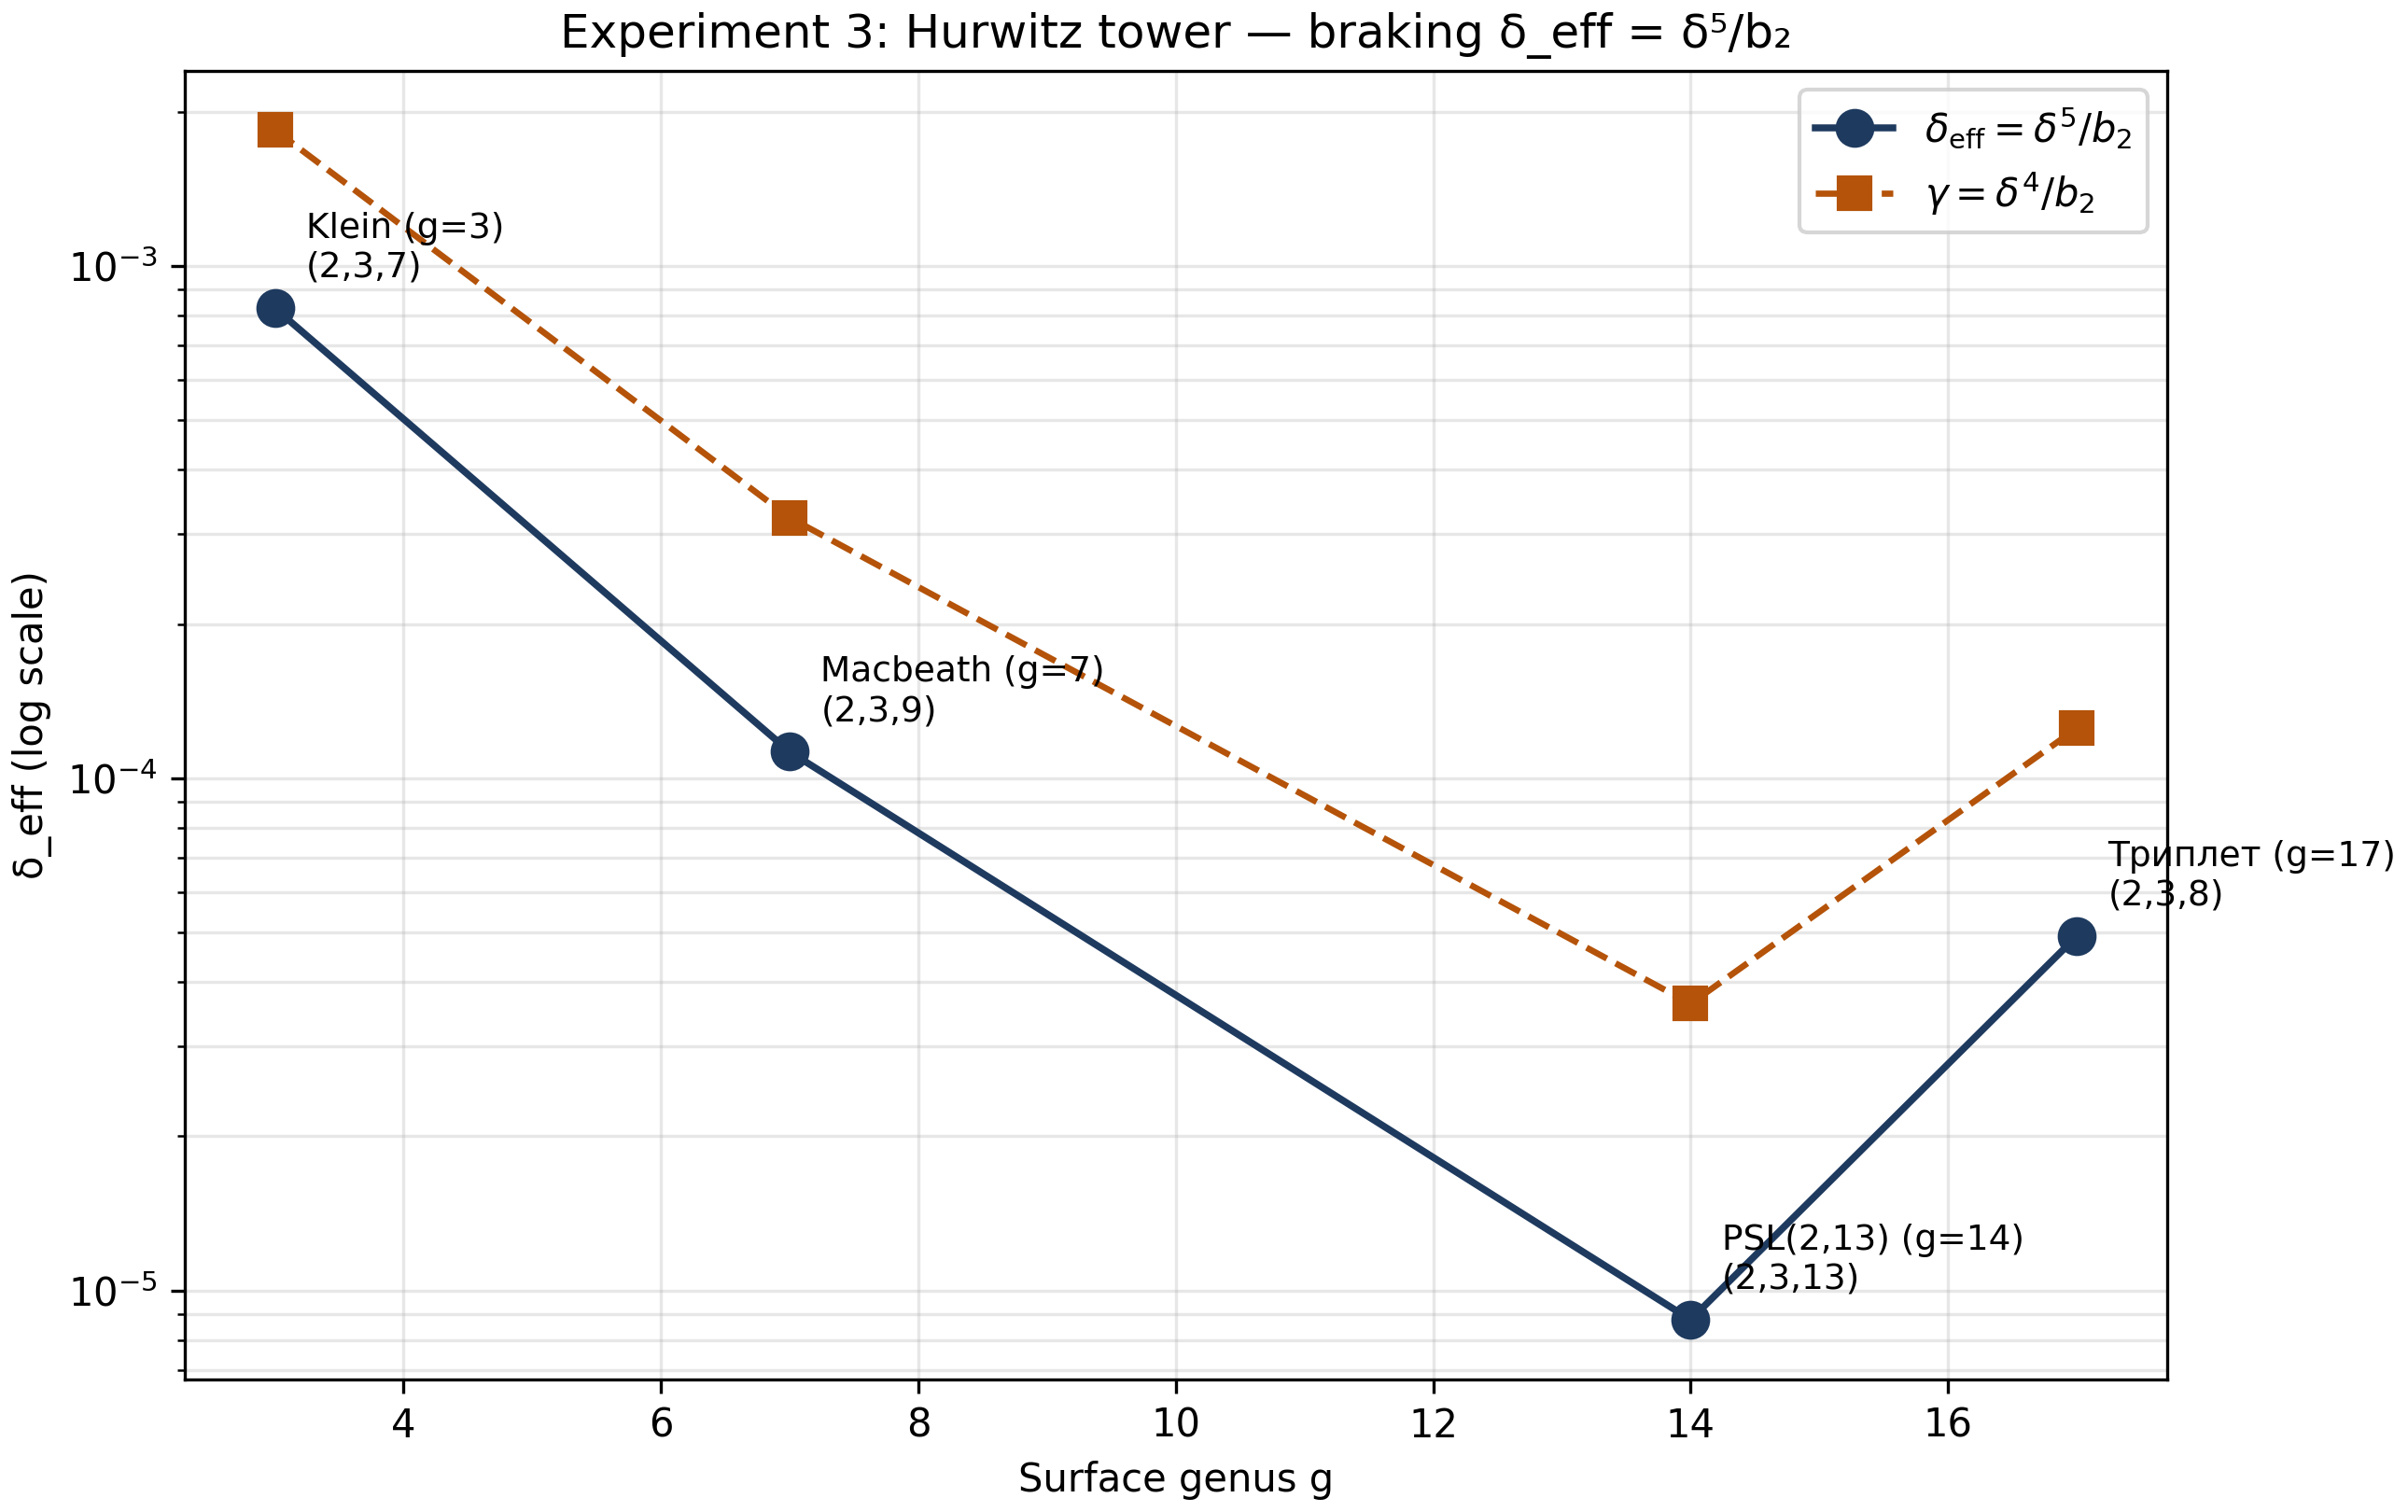
\includegraphics[width=0.8\textwidth]{figures/fig_hurwitz_tower.png}
\caption{Исправленная башня Гурвица (находка D1): строка рода 14 ---
$\mathrm{PSL}(2,13)$, а не невозможная $(g{=}14, n{=}11)$.}
\label{fig:hurwitz}
\end{figure}

\section{Дисциплина честности}\label{sec:honesty}

Каждое утверждение пакета несёт одну из меток: \emph{доказано} (точная
рациональная/целая арифметика), \emph{верифицировано} (машинная
точность, фиксированные сиды), \emph{опровергнуто} (хранится
публично), \emph{гипотеза} (помеченное предположение) --- и живёт в
реестре утверждений с адресом доказательства. Реестр двигается только
на один шаг за раз (открыто $\to$ гипотеза $\to$ верифицировано $\to$
доказано), и опровержения его никогда не покидают. Контракт
воспроизводимости: свежий прогон должен совпасть с закоммиченными
JSON до $10^{-10}$; любое большее отклонение --- находка, и пакет
просит новую строку реестра, а не пересев.

\section{Слой Lean 4}\label{sec:lean}

Точный слой теорем формализован в Lean 4 с Mathlib
(\texttt{dsi\_lab/lean4/}), без sorry: арифметика переписи
($7F = 3V = 2E = 168$, $\chi = -4$), тождество цепных дробей
$9/224 = [0;24,1,8]$, порядок лестницы $5/7 < 1 \le 1 + 2/n \le 2$,
минимум масштабированных перестановок $7(4/7)^2 - 8(4/7) + 3 = 5/7$ и
значение взвешенного дерева $549/49$. Теоремы A/B/C анкерованы
аксиомами: их формулировки точны, численное содержание несут аксиомы,
документированные верифицирующим экспериментом, а следствие~D выведено
из теоремы~A (настоящее доказательство). Аудит аксиом
(\texttt{DSILab\_AxiomAudit.lean}) печатает аксиомный след каждой
теоремы.

\section{Воспроизведение}\label{sec:repro}

\begin{verbatim}
cd dsi_lab
python3 -m pip install -r requirements.txt
make test          # 51+ быстрых теоремных проверок
make validate      # аудит закоммиченных вердиктов
make run           # все 7 экспериментов, детерминизм
make multilang     # кросс-языковой самотест C/C++/JS
\end{verbatim}
Всё работает на Android/Termux без изменений. Переиспользуемое ядро ---
типизированный пакет \texttt{dsilab/}; кросс-языковые двойники ---
\texttt{multilang/} (C, C++, JavaScript байт-в-байт; Rust, Go, Julia
исходники); исходники монографии --- \texttt{monograph/tex/}.

\section*{Литература}
\begin{enumerate}
\item R.~Fricke, F.~Klein, \emph{Vorlesungen \"{u}ber die Theorie der elliptischen Modulfunctionen}, Teubner (1897).
\item J.~Cuntz, \emph{Simple $C^*$-algebras generated by isometries}, Commun.\ Math.\ Phys.\ \textbf{57} (1977).
\item A.~Macbeath, \emph{Generators of the linear fractional groups}, Proc.\ Symp.\ Pure Math.\ \textbf{12} (1969).
\item Родительский репозиторий: \texttt{choptuik\_ac\_bc} --- фреймворк $b$--C/$a$--C, монографии, Einstein Direct, Collapse--Hawking Bridge, QHB, QCD Bridge.
\end{enumerate}

\end{document}
